%%% Section start %%%
\section{Ontological Analysis}
\label{sec-ontology}
According to Guarino ~\cite{ontological-analysis}, “Ontological analysis can be defined as the process of eliciting and discovering relevant distinctions and relationships bound to the very nature of the entities involved in a certain domain, for the practical purpose of disambiguating terms having different interpretations in different contexts.” A good practice here is using a reference ontology, i.e. an explicit and formal representation of a conceptualization of that domain ~\cite{guizzardi:phdthesis05}. Performing an ontological analysis with the use of a reference ontology means interpreting the analyzed domain in terms of the concepts defined in this ontology. This process is aimed at grounding the semantics of the concepts of the domain of interest using the reference ontology. For that, it is paramount to choose a reference ontology of high quality, as this ontology is assumed to be a complete and semantically sound representation of the domain of interest.

In this work, we apply the Decision-Making Ontology (DMO), a well-founded ontology, as the ontological analysis's reference ontology.  Being well-founded means that the concepts of DMO are defined in terms of a foundational ontology (in this case, UFO). As a result, the concepts of DMO have not been defined from scratch. Instead, they have been grounded in the concepts of the foundational ontology, also importing their formal semantics and ontological commitments. This is aimed at making DMO a semantically sound ontology.

In this section, we analyze the definitions of the elements of the GRADE taxonomy and Basic Decision Theory (BDT), that were formally presented in Section~\ref{sec-background}, and evaluate them with the definitions from DMO. Further, we also propose the creation of new concepts or the generalization of existing ones, in order to better explain and represent certain parts of the decision-making domain. 

As we have shown in Section~\ref{sec-background}, the GRADE taxonomy consists of five top-level elements: Goals, Roles, Assets, Decision Methods \& Criteria, and Environment. In turn, each of these elements are further refined in lower-level elements that are intended to represent different perspectives of the top-level ones. However, since the lower-level elements are related to perspectives that are domain-dependent, we will focus only on the top-level ones, which are domain independent, and thus covered by our chosen reference ontology.

In the following subsections, we will use different colors to represent concepts of distinct sources. UFO and DMO concepts are colored in yellow. GRADE concepts are orange. BDT concepts are colored in blue. Finally, new concepts, are presented in green. This decision was made with the goal to clarify where each reused concept fits in our ontology and the new concepts created by it.

%Figure~\ref{fig-colors} presents the types of concepts and their colors.
%\begin{figure}
%	\centering
%	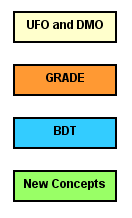
\includegraphics{figuras/fig-colors} 
%	\caption{Presents the types of concepts and the colors that were used.}
%	\label{fig-colors}
%\end{figure}

\subsection{Decision Method and Criteria}

As can be seen in Figure~\ref{fig-decision-making-ontology}, DMO represents both \textit{Criteria} and \textit{Decision} as UML roles, directly connecting \textit{Mental Moment} to Deliberative Act. Here, we prefer to use concepts to represent \textit{Criteria} and \textit{Decision}, because it makes it easier to represent the relation between these concepts and other concepts. 

Although DMO represents the criteria and the result of a decision making, it does not mention the method used in this process. Since this is a concept in the GRADE taxonomy, we suggest the inclusion of the \textit{Decision Method} concept. According to UFO, a decision method can be seen as a \textit{Complex Action Universal}, i.e. a process that will be followed by someone when taking a decision. We define it as a Universal (i.e. type) rather than an Particular (i.e. instance), because the method defines in the type level, the set of activities to be followed. In this sense, the \textit{Deliberative Act} may be seen as a instance of the \textit{Decision Method}.

Figure~\ref{fig-ontology-criteria-decision-method2} presents the new concepts that are being proposed.
\begin{figure}
	\centering
	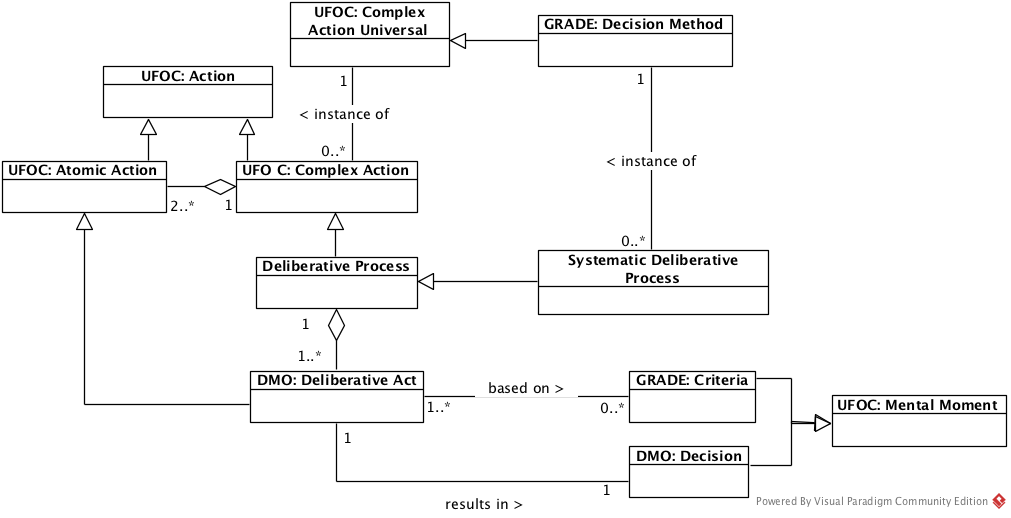
\includegraphics[width=\textwidth]{figuras/deliberative-process}
	\caption{Fragment of the Ontological Analysis that represents the \textit{Decision Method} and the \textit{Criteria}}
	\label{fig-ontology-criteria-decision-method2}
\end{figure}


\subsection{Roles}

The only role (in the sense of UFO-C:Agent) considered in DMO is the \textit{Decision Maker}, GRADE, on the other hand, considers other roles for people which are involved in the decision-making. These Decision Stakeholders are \textit{Agents} (persons, groups or even organizations) who, in some way, influence decision-making process. We will consider that this "influence" is to give a \textit{Criteria} that will base the \textit{Decision Method}. Therefore, every \textit{Criteria} is given by a \textit{Decision Stakeholder}, which in turn assigns a value to that \textit{Criteria}. It means that the \textit{Decision Stakeholder} performs an \textit{Evaluation} using the criteria. In its turn, the \textit{Decision Maker} is, a specific type of \textit{Decision Stakeholder} that makes the final decision (and that is considered responsible by it). For example, during the World War II, Winston Churchill said: "\textit{Gentlemen, what I expect from you is that after a reasonable amount of time and discussion, everyone in this room will agree with me}". In this example, Churchill made clear that although there were many \textit{Decision Stakeholders} in the room, he is the \textit{Decision Maker}, responsible for the \textit{Deliberative Act}. Finally, it is important to mention that each \textit{Criteria} can be evaluated for different value perspectives.

Figure~\ref{fig-ontology-decision-stakeholder} presents the relations between the \textit{Decision Stakeholder} and the \textit{Criteria}.

\begin{figure}
	\centering
	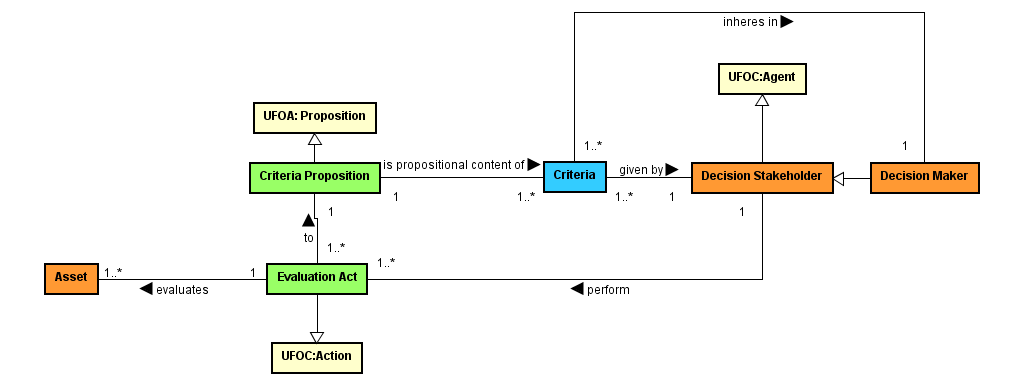
\includegraphics[width=\textwidth]{figuras/fig-ontology-decision-stakeholder} 
	\caption{Fragment of the Ontological Analysis that presents the concept of \textit{Decision Stakeholder}.}
	\label{fig-ontology-decision-stakeholder}
\end{figure}


\subsection{Assets}

The GRADE taxonomy is not clear about the definition of \textit{Asset}, however, it gives us some examples of assets (hardware, software or systems composed by hardware and software) that allow us to infer that \textit{Asset} is a type of \textit{Object}.   Moreover, in an GRADE application , \textit{Assets} can be considered architectural options in the decision making, thus, comparable to Acts in TBD, with the difference that in TBD the options are more generic since it is in an domain-independent decision-making process. In this work we opted for use the word "Option" instead of "Acts" to name the concept that represents the options considered in a decision making. So \textit{Option} is an \textit{Individual} (can be a \textit{Endurant} like a software or an \textit{Perdurant} like an Action to be performed by the Decision Maker) considered by the \textit{Decision Maker} as an possible result in a \textit{Deliberative Act}.
It should also be noted that being an \textit{Asset} by itself is not sufficient cause for this \textit{Asset} to be in a decision-making context. It will only be in this context if it is indicated as an option in a decision-making process by a \textit{Decision Stakeholder}. Moreover, this \textit{Option} is indicated by an \textit{Action} defined as \textit{Option Indication}, which is performed by a \textit{Decision Stakeholder}.

Figure~\ref{fig-ontology-assets} presents a fragment of our ontology that represents the ontological nature of \textit{Assets}.


\begin{figure}
	\centering
	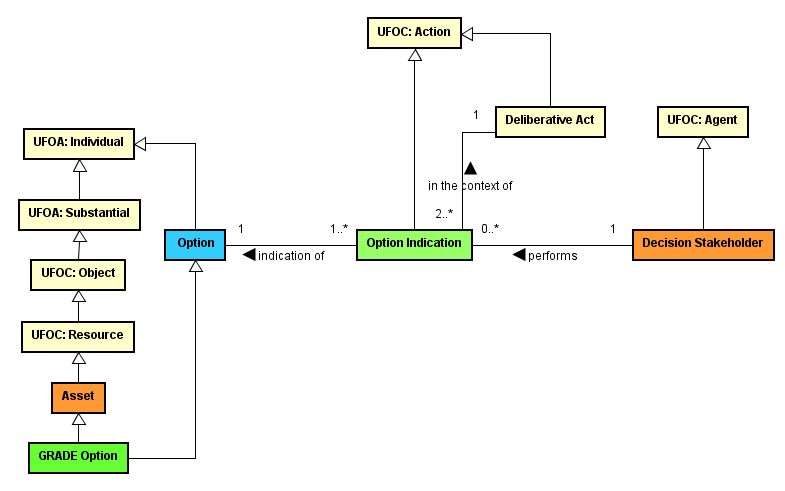
\includegraphics[width=\textwidth]{figuras/fig-ontology-assets} 
	\caption{Ontology fragment that contemplates concepts of \textit{Asset} and \textit{Option}.}
	\label{fig-ontology-assets}
\end{figure}

An \textit{Option} is created in an indication (\textit{Option Indication}) by a \textit{Stakeholder}. Each indication creates an \textit{Expectation} that, if chosen, it will result in a possible situation. It is similar to "Outcome" in BDT. This \textit{Expectation} will influence the decision making thus it is a type of \textit{Criteria}.

Each \textit{Criteria} has its propositional content evaluated (\textit{Evaluation}) by the \textit{Decision Stakeholder} who indicates it. This \textit{Evaluation} is similar to "Payoff" in BDT.

Figure~\ref{fig-evaluate-indication} presents a fragment of our ontology that represents the evaluation of \textit{Option}.


\begin{figure}
	\centering
	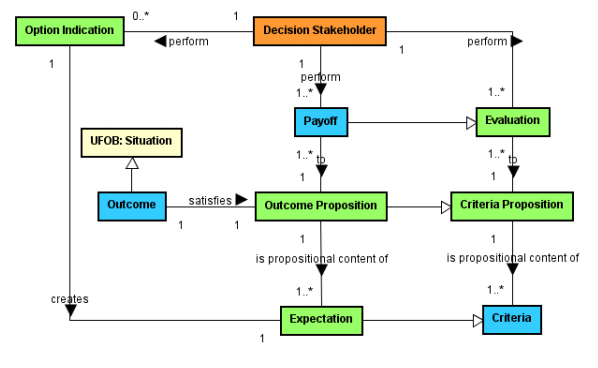
\includegraphics[width=\textwidth]{figuras/fig-evaluate-indication} 
	\caption{Ontology fragment that contemplates concepts of \textit{Option} and \textit{Evaluation}.}
	\label{fig-evaluate-indication}
\end{figure}

\subsection{Goals}

It is clear that \textit{Goals}, \textit{Intentions} and even \textit{Beliefs} of a \textit{Decision Maker} can influence his Decisions. Because of that, we have a type of Criteria that is associated with that goal. The concepts of \textit{Goal} and \textit{Intention} of UFO-C can be associated with the concept of Goal in GRADE. However, a \textit{Goal} in UFO-C extrapolates the decision context, that is, not every instance of \textit{Goal} is associated with a instance of \textit{Deliberative Act}. This association occurs through a particular type of \textit{Intention}. Therefore, we propose the creation of two new concepts: \textit{Decision Goal} and \textit{Decision Intention} with the following definitions:
Decision Intention: This is a type of \textit{Criteria} and \textit{Intention} that represents the purpose of the \textit{Decision Maker}.
Decision Goal: It is a \textit{Goal} that is the propositional content of a \textit{Decision Intention}.

Figure~\ref{fig-ontology-goals} presents a fragment of our ontology that represents a \textit{Goal} and its relations.

\begin{figure}
	\centering
	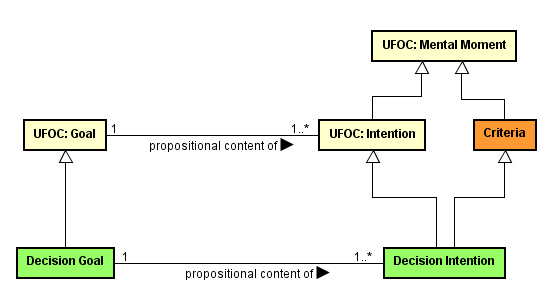
\includegraphics[width=\textwidth]{figuras/fig-ontology-goals} 
	\caption{Ontology fragment that contemplates the concept of \textit{Goal}.}
	\label{fig-ontology-goals}
\end{figure}

Each \textit{Criteria} has your proposition content evaluated by the \textit{Decision Stakeholder} who indicates it. The GRADE indicates a list of value perspectives under which the Goals can be evaluated. In this work, we represent these perspectives as generalizations of the new concept \textit{Goal Value Perspective}. In other words, \textit{Goal Value Perspectives} are \textit{Value Perspectives} in the context of a \textit{Goal Evaluation} and a \textit{Goal Evaluation} is an \textit{Evaluation} of a \textit{Decision Goal}.

Figure~\ref{fig-goal-evaluation} presents a fragment of our ontology that represents a \textit{Goal Evaluation} and \textit{Goal Value Perspective}.

\begin{figure}
	\centering
	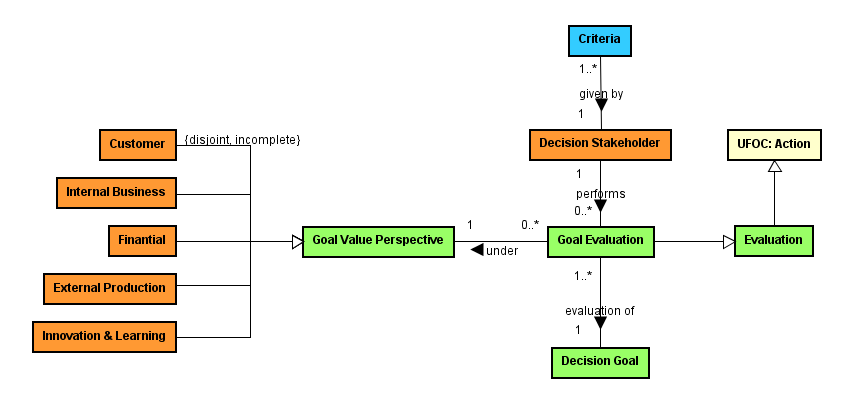
\includegraphics[width=\textwidth]{figuras/fig-goal-evaluation} 
	\caption{Ontology fragment that represents a \textit{Goal Evaluation} and its relations.}
	\label{fig-goal-evaluation}
\end{figure}


\subsection{Environment}


In GRADE, \textit{Environment} is defined as a fact that is in the context of the decision but beyond the control of \textit{Decision Maker}. In this sense, we can understand a "fact" as a portion of reality that exists in its own. This is exactly the definition of \textit{Situation} in UFO-A. In~\cite{guizzardi-et-al:er13}, Guizzardi proposes a theory where \textit{Situations}, as states of affairs, can be divided in "Factual", which are Situations that are obtained at a time point (e.g the situation where Donald Trump is president of the United States) and "Counterfactual", which never are obtained in a time point. Because of that, we propose that the concept of \textit{Environment} should be renamed to \textit{Environmental Fact} and understood as a factual \textit{Situation}, as it is defined in UFO and used in DMO. In other words, they represent a portion of the reality, prior to the \textit{Deliberative Act}. Besides that, in this work, we propose that what influences the decision are \textit{Mental Moments} (\textit{Criteria}). Therefore, we created the concepts of \textit{Environment Proposition}, which is an abstract representation of the \textit{Environment}, based on a moment of the \textit{Decision Maker}. Finally, it is important to explain that, as it is defined in UFO, after the occurrence of an \textit{Event//Action} (in this case, the \textit{Deliberative Act}) a new Situation will be brought into existence, the one that was created by the occurrence of \textit{Deliberative Act}, however this new situation cannot be considered a \textbf{post-state} \textit{Environment}, since it would violate the definition that is presented in the taxonomy.


Figure~\ref{fig-ontology-environment} presents the ontological nature of the concept \textit{Environment}.

\begin{figure}
	\centering
	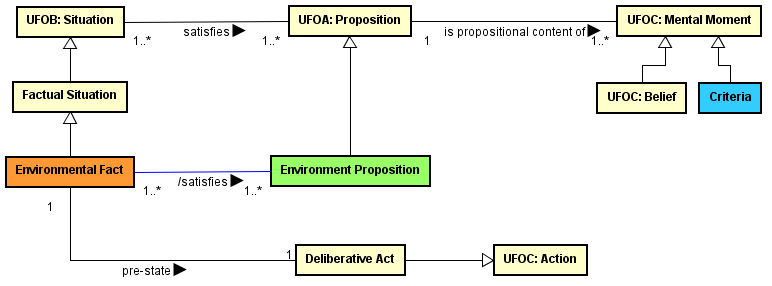
\includegraphics[width=\textwidth]{figuras/fig-ontology-environment} 
	\caption{Fragment of the Ontological Analysis that presents the concept \textit{Environment}.}
	\label{fig-ontology-environment}
\end{figure}